\section{Réglage des hyper-paramètres}%
\label{sec.results.hparams}

Les résultats présentés dans Section~\ref{sub.results.training.results} sont satisfaisants.
Il n'est donc pas strictement nécessaire d'effectuer un réglage des hyperparamètres.
Cependant, il est possible en le faisant d'obtenir des résultats comparables 
en moins d'époques ou avec un modèle plus petit.
Pour cette raison, nous avons décidé de l'entamer.

\subsection{Configuration}%
\label{sub.results.hparams.config}

Nous avons fait le choix de restreindre la portée de ce réglage à deux hyperparamètres :
le taux d'apprentissage (\(\eta\) ou \verb|lr|) et le (\verb|dropout|).
Nous avons opté pour une recherche Bayésienne avec des lois \(\log\)--uniformes sur les intervalles
\(\left[10^{-5}, 10^{-1}\right]\) et \([0.1, 0.5]\) respectivement.
Les autres hyperparamètres ont été fixés à leurs valeurs données dans Section~\ref{sub.results.training.hyperparameters}.

Pour chaque combinaison de \verb|lr| et \verb|dropout|, nous avons entraîné le modèle pendant 2 époques.
L'objectif de la recherche est de maximiser le score \gls{bleu} sur le corpus de validation.
Nous avons limité le nombre d'essais à 20.

\subsection{Résultats}%
\label{sub.results.hparams.results}

Les 20 essais ont été effectués en 2h 17m 13s 11ms.
Les résultats sont présentés dans Figure~\ref{fig.results.hparams}.
\begin{figure}[hbt]
    \centering
    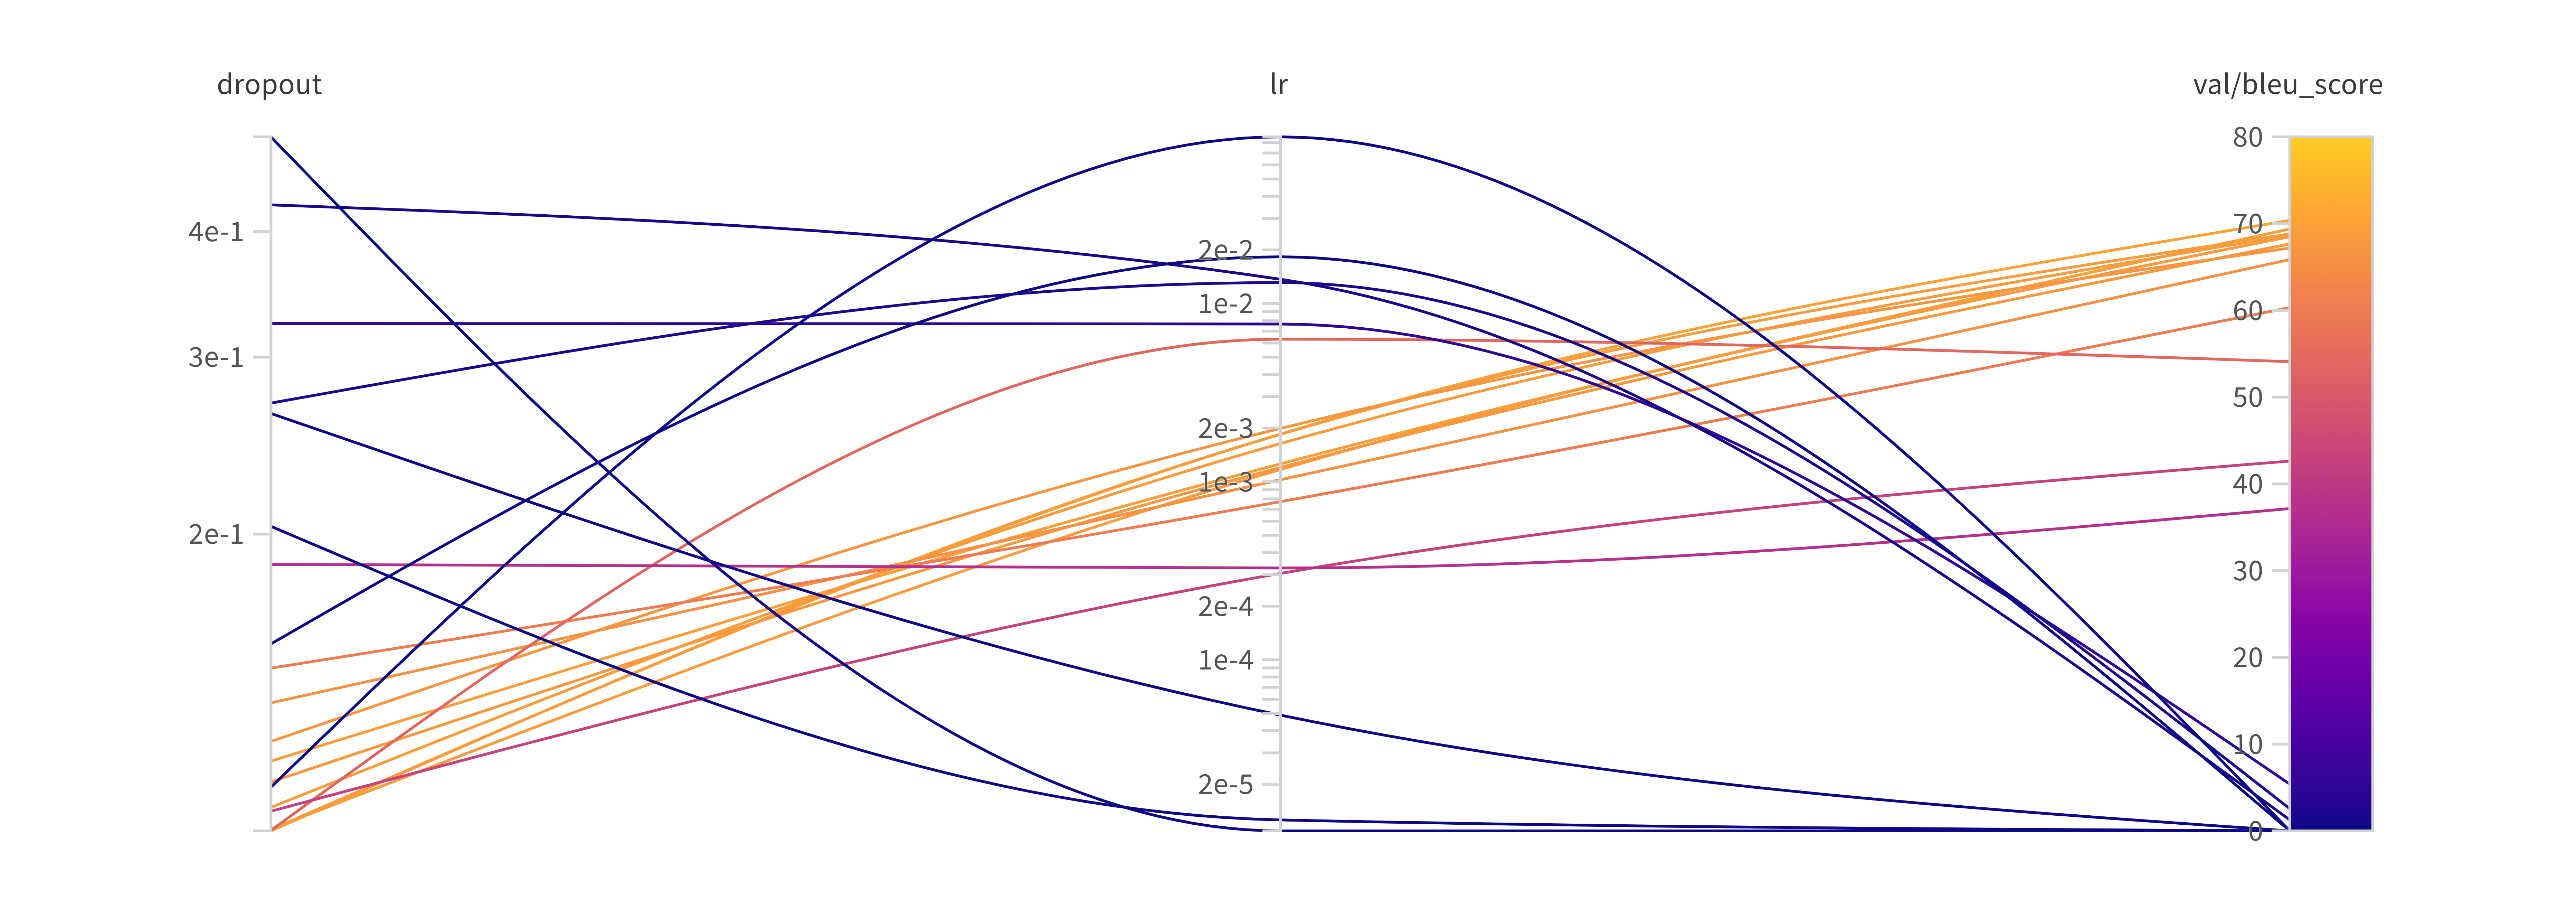
\includegraphics[width=.8\textwidth]{assets/images/sweep.png}
    \caption{Résultats de la recherche Bayésienne des hyperparamètres.}%
    \label{fig.results.hparams}
\end{figure}
La figure en question est une visualisation en coordonnées parallèles des résultats.
L'axe de gauche représente la valeur de \verb|dropout| sur une échelle linéaire, 
celui du milieu la valeur de \verb|lr| sur une échelle logarithmique 
et celui de droite le score \gls{bleu} sur une échelle de 0 à 100.
Un essai est représenté par une courbe qui relie les 3 points correspondants sur les 3 axes.
La couleur de la courbe indique le score \gls{bleu} associé.
Elle est interpolée entre le violet (0\%) et l'orange (100\%).
Les mêmes informations sont présentes dans Table~\ref{tab.results.hparams} sous forme numérique.

\begin{table}[htb]
    \begin{center}
        \adjustbox{max width=\linewidth}{
            \begin{tabular}{l*{20}{c}}
                \toprule
                \verb|dropout|        
                &  0.26 &  0.16 &  0.32 &  0.19 &  0.10 &  0.10 &  0.11 &  0.11 &  0.50 &  0.12 &  0.11 &  0.12 &  0.11 
                &  0.10 &  0.10 &  0.14 &  0.27 &  0.15 &  0.20 &  0.43 \\
                \verb|lr| \((\log_{10})\)
                & -4.31 & -1.74 & -2.12 & -3.48 & -2.73 & -2.73 & -2.92 & -1.06 & -4.96 & -2.90 & -2.79 & -2.70 & -3.52 
                & -2.20 & -2.93 & -2.99 & -1.88 & -3.11 & -4.90 & -1.86 \\
                \midrule
                \verb|val/bleu| (\%)
                &  0.00 &  0.00 &  5.39 & 37.15 & 68.80 & 70.37 & 67.66 &  0.00 &  0.00 & 69.37 & 68.68 & 67.19 & 42.63 
                & 54.09 & 68.49 & 65.85 &  2.55 & 60.32 &  0.00 &  1.26 \\
                \bottomrule
            \end{tabular}
        }
    \end{center}
    \caption{Résultats de la recherche Bayésienne des hyperparamètres.}%
    \label{tab.results.hparams}
\end{table}

On observe sur la figure un regroupement des lignes oranges (les meilleurs essais) 
dans la région qui correspond à \verb|dropout| \(\in[0.1, 0.15]\) et \(\eta\approx 10 ^{-3}\).
Cela est aussi apparent sur le tableau.
\begin{table}[hbt]
    \begin{center}
        \begin{tabular}{|l|c|c|}
            \cline{2-3}
            \multicolumn{1}{c|}{} & Importance & Corrélation \\
            \hline
            \verb|dropout|        & 63.9\%     & - 0.899     \\
            \hline
            \verb|lr|             & 36.1\%     & - 0.647     \\
            \hline
        \end{tabular}
    \end{center}
    \caption{Importance et corrélation des hyperparamètres.}
    \label{tab.results.hparam.corr}
\end{table}
Une analyse factorielle sur les essais effectués nous permet d'estimer l'importance des hyperparamètres 
ainsi que leurs corrélations avec le score \gls{bleu}.
Ils sont tous deux négativement corrélés avec ce dernier.
Le \verb|dropout| est le plus important entre les deux (voir Table~\ref{tab.results.hparam.corr}).
La meilleure valeur du score \gls{bleu} est obtenue 
avec \verb|dropout| \(\approx 0.101599\) et \(\eta\approx 0.0018488801\).
Pour cette valeur, le score \gls{bleu} sur le corpus de validation est de 70.37\% après 2 époques.